% Options for packages loaded elsewhere
\PassOptionsToPackage{unicode}{hyperref}
\PassOptionsToPackage{hyphens}{url}
%
\documentclass[
]{book}
\usepackage{amsmath,amssymb}
\usepackage{lmodern}
\usepackage{iftex}
\ifPDFTeX
  \usepackage[T1]{fontenc}
  \usepackage[utf8]{inputenc}
  \usepackage{textcomp} % provide euro and other symbols
\else % if luatex or xetex
  \usepackage{unicode-math}
  \defaultfontfeatures{Scale=MatchLowercase}
  \defaultfontfeatures[\rmfamily]{Ligatures=TeX,Scale=1}
\fi
% Use upquote if available, for straight quotes in verbatim environments
\IfFileExists{upquote.sty}{\usepackage{upquote}}{}
\IfFileExists{microtype.sty}{% use microtype if available
  \usepackage[]{microtype}
  \UseMicrotypeSet[protrusion]{basicmath} % disable protrusion for tt fonts
}{}
\makeatletter
\@ifundefined{KOMAClassName}{% if non-KOMA class
  \IfFileExists{parskip.sty}{%
    \usepackage{parskip}
  }{% else
    \setlength{\parindent}{0pt}
    \setlength{\parskip}{6pt plus 2pt minus 1pt}}
}{% if KOMA class
  \KOMAoptions{parskip=half}}
\makeatother
\usepackage{xcolor}
\IfFileExists{xurl.sty}{\usepackage{xurl}}{} % add URL line breaks if available
\IfFileExists{bookmark.sty}{\usepackage{bookmark}}{\usepackage{hyperref}}
\hypersetup{
  pdftitle={MBAn Career Handbook},
  pdfauthor={Team - Keep Rolling},
  hidelinks,
  pdfcreator={LaTeX via pandoc}}
\urlstyle{same} % disable monospaced font for URLs
\usepackage{longtable,booktabs,array}
\usepackage{calc} % for calculating minipage widths
% Correct order of tables after \paragraph or \subparagraph
\usepackage{etoolbox}
\makeatletter
\patchcmd\longtable{\par}{\if@noskipsec\mbox{}\fi\par}{}{}
\makeatother
% Allow footnotes in longtable head/foot
\IfFileExists{footnotehyper.sty}{\usepackage{footnotehyper}}{\usepackage{footnote}}
\makesavenoteenv{longtable}
\usepackage{graphicx}
\makeatletter
\def\maxwidth{\ifdim\Gin@nat@width>\linewidth\linewidth\else\Gin@nat@width\fi}
\def\maxheight{\ifdim\Gin@nat@height>\textheight\textheight\else\Gin@nat@height\fi}
\makeatother
% Scale images if necessary, so that they will not overflow the page
% margins by default, and it is still possible to overwrite the defaults
% using explicit options in \includegraphics[width, height, ...]{}
\setkeys{Gin}{width=\maxwidth,height=\maxheight,keepaspectratio}
% Set default figure placement to htbp
\makeatletter
\def\fps@figure{htbp}
\makeatother
\setlength{\emergencystretch}{3em} % prevent overfull lines
\providecommand{\tightlist}{%
  \setlength{\itemsep}{0pt}\setlength{\parskip}{0pt}}
\setcounter{secnumdepth}{5}
\usepackage{booktabs}
\ifLuaTeX
  \usepackage{selnolig}  % disable illegal ligatures
\fi
\usepackage[]{natbib}
\bibliographystyle{apalike}

\title{MBAn Career Handbook}
\author{Team - Keep Rolling}
\date{2022-08-03}

\begin{document}
\maketitle

{
\setcounter{tocdepth}{1}
\tableofcontents
}
\hypertarget{homepage-of-the-book}{%
\chapter*{HomePage of the Book}\label{homepage-of-the-book}}
\addcontentsline{toc}{chapter}{HomePage of the Book}

\begin{quote}
You are expected to Build the whole book and not just Knit the Homepage.Need to add few things here.
\end{quote}

\hypertarget{motivation-for-the-book}{%
\chapter*{Motivation for the book}\label{motivation-for-the-book}}
\addcontentsline{toc}{chapter}{Motivation for the book}

\begin{quote}
This handbook is for current and future MBAn students to understand how the program works, what the targeted jobs are, and how to prepare for recruiting processes. The handbook will first begin with an overview of the MBAn program, describing different resources available from the Ross experience, classes you may take, and the skills gained from it. Following this introduction, we will transition into the main section of the book, detailing career outcomes available to MBAn students, driven by research from other school's Business Analytics program, the CDO resources, and experiences from former Master of Management students that have moved onto careers. We will introduce techniques for going through career exploration independently while utilizing the guide. Next will be a chapter focusing on the overall recruiting process for the discussed careers and how MBAn students can prepare and plan for networking, applications, and interviews. We will accumulate best practices for resumes, cover letters, and interviews. A final section will be included detailing supportive resources for the challenges international students face when searching for careers in the U.S. and globally, including a dynamic list of companies that offer sponsorship. We recognize research and resources our team is able to provide over the next few weeks is non-exhaustive, but we hope for this handbook to be a baseline for future students of this program and can live on and be updated in the future as the Master of Business Analytics Graduates enter the workforce and find success in their careers.
\end{quote}

\hypertarget{about-us}{%
\chapter{About Us}\label{about-us}}

We are Team Keep Rolling, a group of MBAn students in the first-ever year of this new program! We chose this name to describe us because we went into this semester with the plan to never give up, continue to be creative and bring our ideas together for success!

\includegraphics[width=0.5\textwidth,height=\textheight]{Images/group_pic.png}

As individuals, we bring lots of different skills and perspectives to this collective team and are motivated to learn more about career paths for this new program to serve future students. You can learn more about each of us in the sections to follow.

\hypertarget{amey-bhile}{%
\section{Amey Bhile}\label{amey-bhile}}

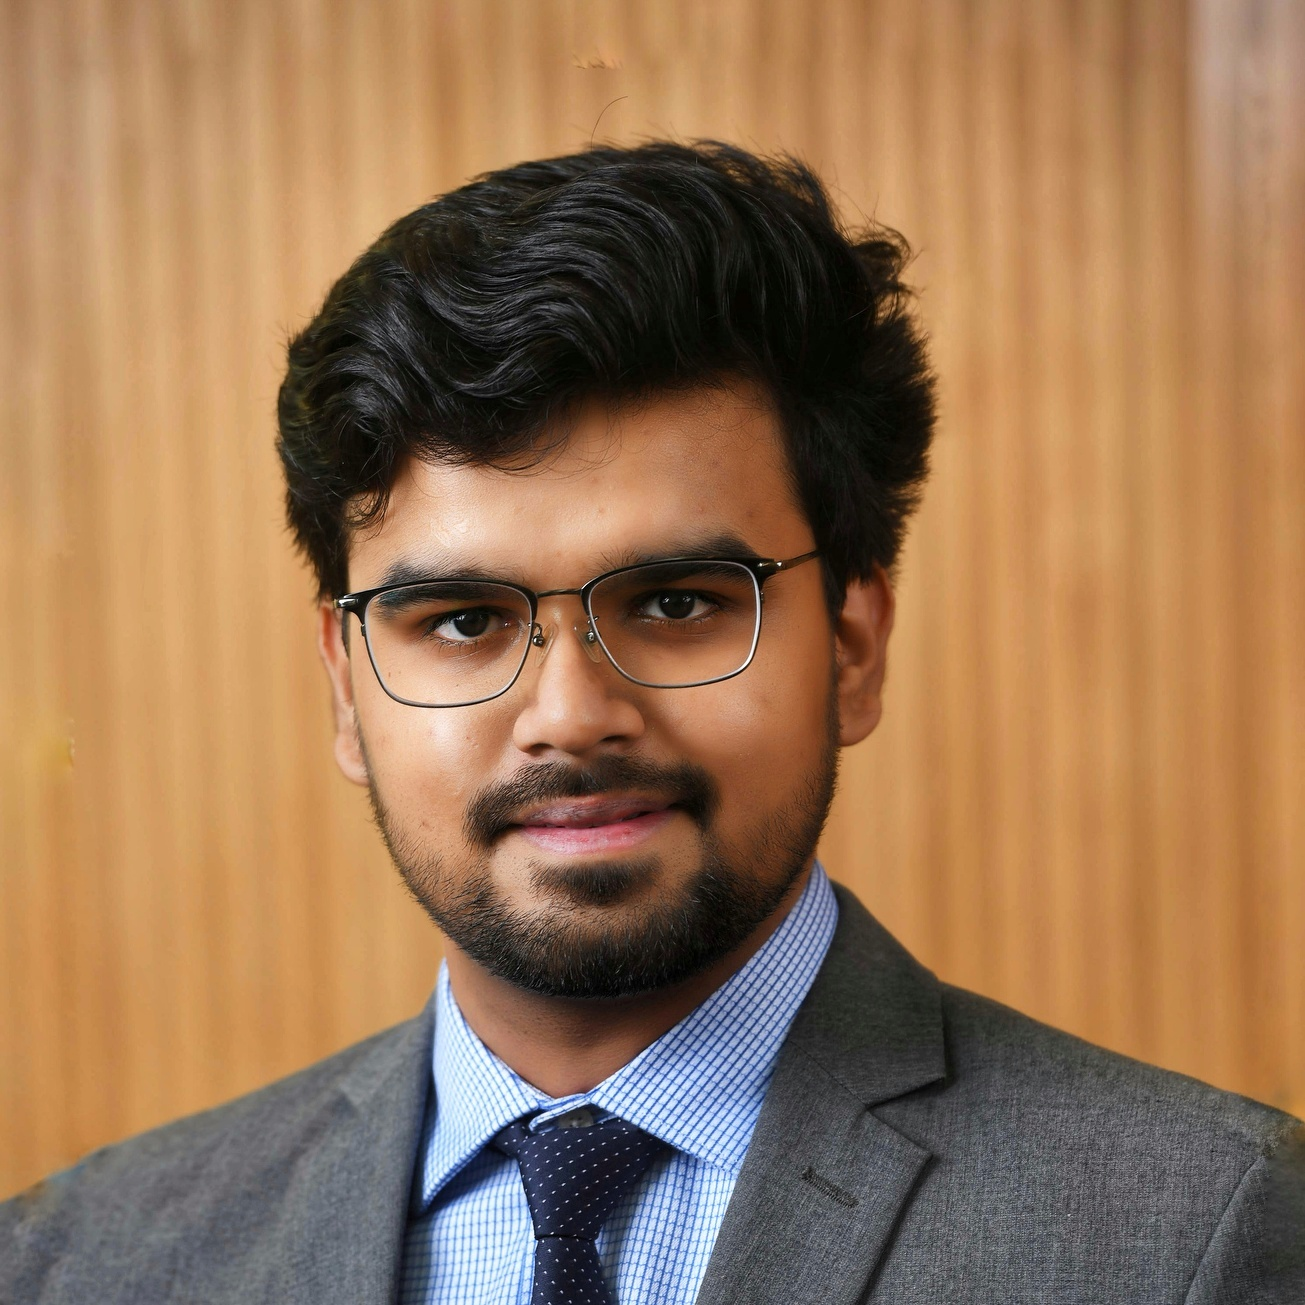
\includegraphics[width=0.5\textwidth,height=\textheight]{Images/Amey.jpeg}

\begin{quote}
Hey There, MBAn folk !! I'm Amey\\
I was born and brought up in India, where I also completed my Bachelor of Engineering in Computer Science, after which I worked as a technology consultant for three years. During my time at Deloitte, I realized my interests lie at the interface of technology and business; And I needed to expand my skills and knowledge in these domains, which is when I decided to join Ross Business School. ~
I wish to leverage data and apply ML/analytical frameworks to derive actionable insights and create value. I enjoy operating far outside my comfort zone and believe in the power of incremental improvements.\\
Feel free to reach out; I am always happy to help :)
\end{quote}

\begin{quote}
``Data is just summaries of thousands of stories - tell a few of them to the world, and you are a data analyst.''
\end{quote}

\hypertarget{eunguy-lee}{%
\section{Eunguy Lee}\label{eunguy-lee}}

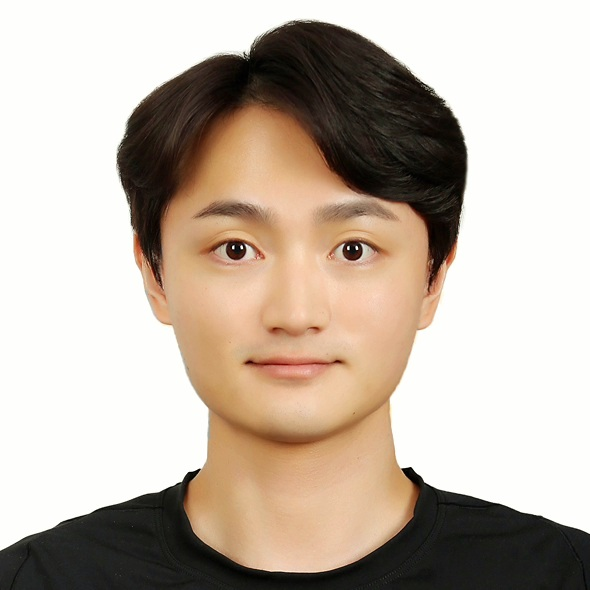
\includegraphics[width=0.5\textwidth,height=\textheight]{Images/Eunguy.jpg}

\begin{quote}
Hello everyone! This is Eunguy.\\
I was born in 1996 and grew up in South Korea. I went to Michigan State University and studied Supply Chain Management. After my junior year in college, I went back to South Korea to serve military as an operations sergeant for about two years. After the military experience, I finished my bechelor degree with online courses from MSU because of the pandemic. Meanwhile, I felt the need of capability handling data so I applied for graduate school with Business Analytics major.
\end{quote}

\begin{quote}
At this point at Ross, I am so exciting to build my network and equip myself with useful tools, such as Python, R, and SQL. As a business person, I am not used to these computer skills. However, someone said ``the pain that doesn't kill you will make you stronger.'' I believe putting my time and effort for the next 10 months will develop my ability as a business analyst. I hope this career handbook brings some insights for you.
\end{quote}

\hypertarget{snow-shen}{%
\section{Snow Shen}\label{snow-shen}}

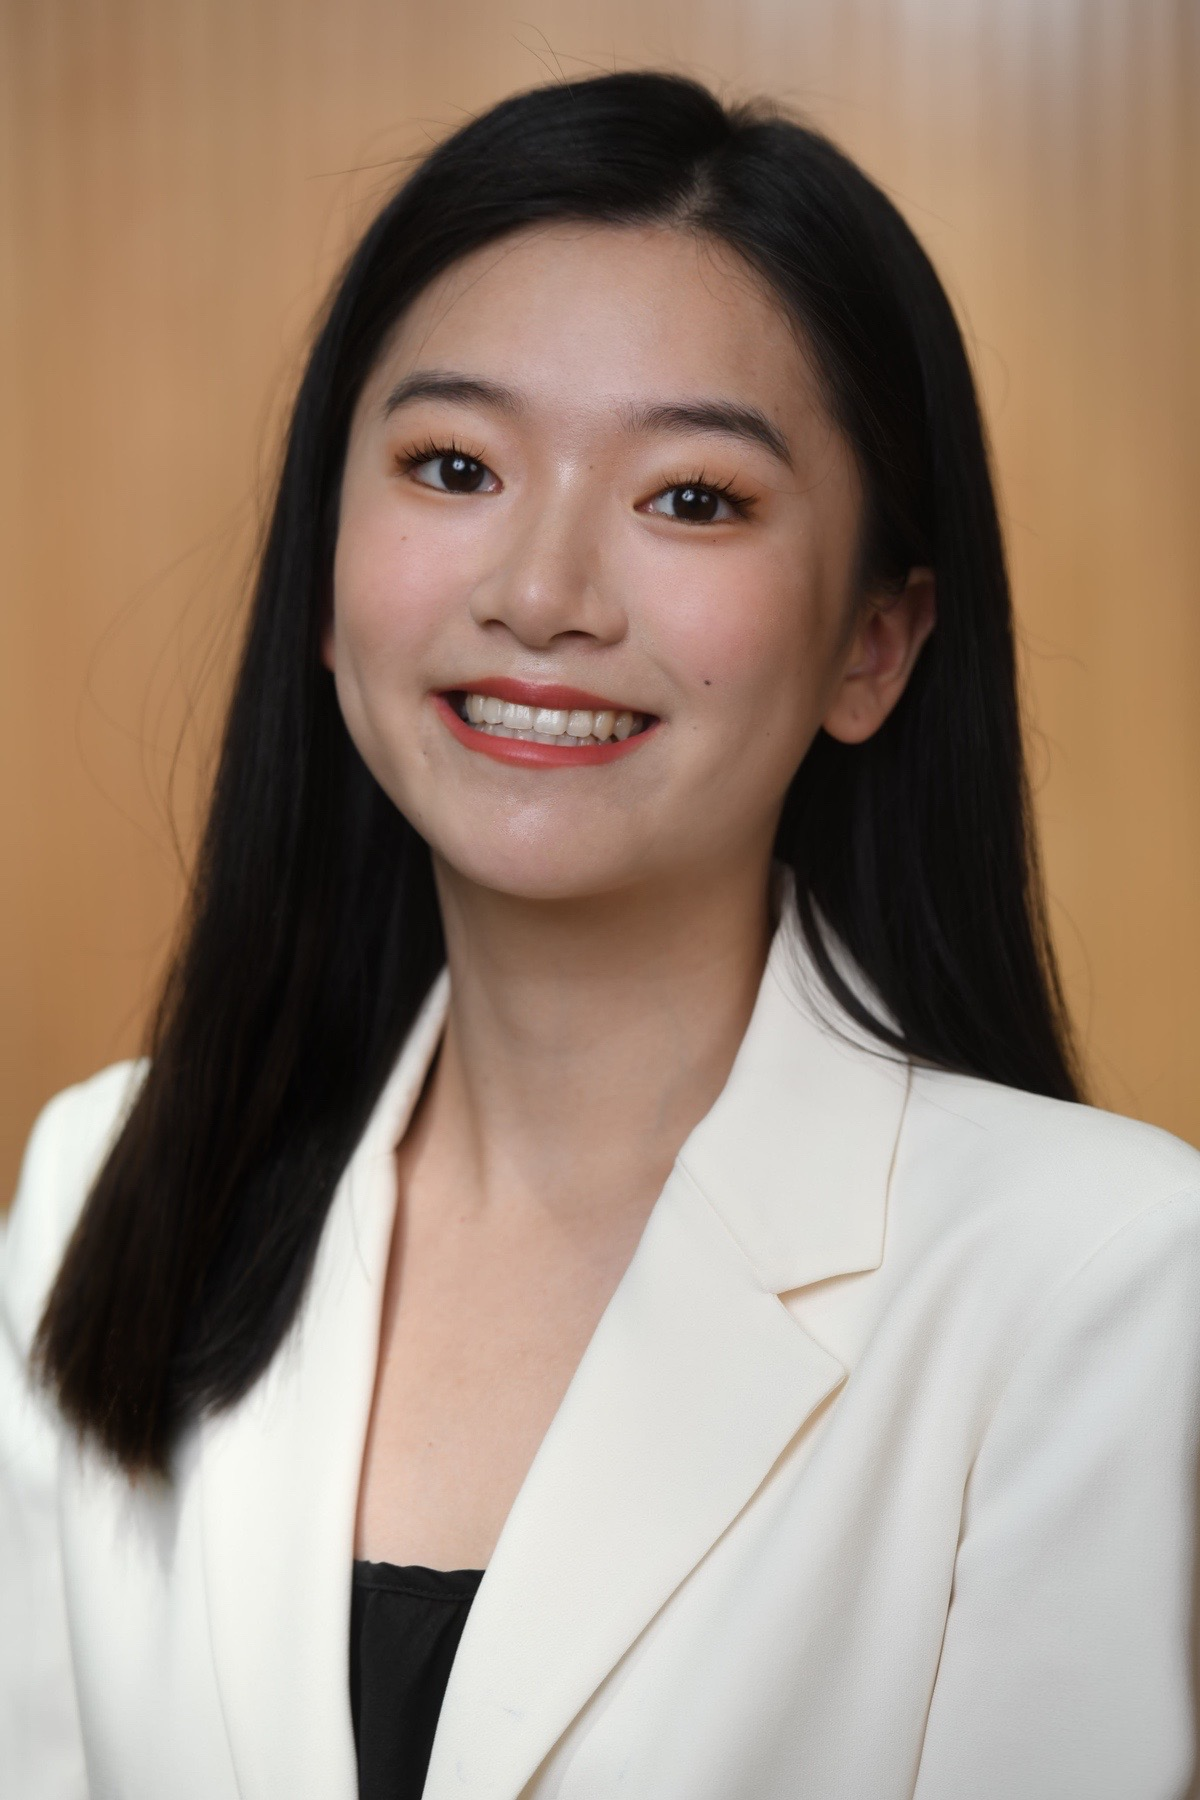
\includegraphics[width=0.5\textwidth,height=\textheight]{Images/Snow.png}

\begin{quote}
Hi, I'm Snow! I come from a southern city in China called Hangzhou. It's warm there and seldomly snows. Every winter, I waited for snow and hoped the world can be covered in white when I wake up. That's why my parents gave me the English name Snow. I went to US in 2019 for my undergrad study. Boston was my destination due to the attractiveness of snow. I spent three years at Boston and then moved to Ann Arbor for graduate study. People hate the long winter here, but I am looking forward to it!
\end{quote}

\hypertarget{mary-silvio}{%
\section{Mary Silvio}\label{mary-silvio}}

\includegraphics[width=0.5\textwidth,height=\textheight]{Images/Mary.JPEG}

\begin{quote}
I am a self-proclaimed true Midwestern girl that grew up in Livonia, Michigan (perfectly halfway between Ann Arbor and Detroit). I graduated from the University of Michigan College of Engineering in Spring 2022 with a B.S.E. in Chemical Engineering and am a current Master's of Business Analytics student at the Stephen M. Ross School of Business. If there is one thing I took away from my undergraduate years, it is that the world will never run out of ways to improve, and thus never run out of problems to solve. Pushing the bounds of knowledge is what allows us to improve the systems around us, and that is why I value the potential of harnessing data - bringing me to the MBAn program to build my analytic skills to give data power.
\end{quote}

\begin{quote}
I have experience working in Chemical Manufacturing, Engineering Research, and Higher Education. Outside of school, I love going to SoulCycle, going on walks with friends, watching Detroit sports, trying new coffee shops, and cooking! It is my dream to be an analyst by day, and cycling instructor by night.
\end{quote}

\hypertarget{ziye-wang}{%
\section{Ziye Wang}\label{ziye-wang}}


\includegraphics[width=0.5\textwidth,height=\textheight]{Images/Siye.jpg}

\begin{quote}
My name is Ziye Wang, from Beijing, China. I graduated from the Central University of Finance and Economics in China, majoring in Financial Engineering.After graduation, I joined Capgemini Invent as an associate consultant, focused on auto and digital transformation.
\end{quote}

\begin{quote}
Something interesting about me I'd like to share with you:
I like drinking more than I like soup
I have 3 cute little nephews and my favorite thing to do on weekends is to play with my little nephew
I'm a Cancer girl but I'm more of a Leo
I lost weight for 5 years but never succeeded
\end{quote}

\begin{quote}
I'm very happy to be part of the Ross community. Hopefully our work will be helpful to everyone.
\end{quote}

\hypertarget{why-choose-the-mban-program-at-ross}{%
\chapter*{Why Choose the MBAn Program at Ross?}\label{why-choose-the-mban-program-at-ross}}
\addcontentsline{toc}{chapter}{Why Choose the MBAn Program at Ross?}

\hypertarget{program-value}{%
\section{Program Value}\label{program-value}}

\hypertarget{coursework}{%
\section{Coursework}\label{coursework}}

\hypertarget{career-resources}{%
\section{Career Resources}\label{career-resources}}

\hypertarget{career-development-office}{%
\subsection{Career Development Office}\label{career-development-office}}

\hypertarget{other-ross-resources}{%
\subsection{Other Ross Resources}\label{other-ross-resources}}

\hypertarget{long-term-gains}{%
\section{Long-Term Gains}\label{long-term-gains}}

\hypertarget{parts}{%
\chapter{Parts}\label{parts}}

You can add parts to organize one or more book chapters together. Parts can be inserted at the top of an .Rmd file, before the first-level chapter heading in that same file.

Add a numbered part: \texttt{\#\ (PART)\ Act\ one\ \{-\}} (followed by \texttt{\#\ A\ chapter})

Add an unnumbered part: \texttt{\#\ (PART\textbackslash{}*)\ Act\ one\ \{-\}} (followed by \texttt{\#\ A\ chapter})

Add an appendix as a special kind of un-numbered part: \texttt{\#\ (APPENDIX)\ Other\ stuff\ \{-\}} (followed by \texttt{\#\ A\ chapter}). Chapters in an appendix are prepended with letters instead of numbers.

\hypertarget{why-choose-the-mban-program-at-ross-1}{%
\chapter{Why Choose the MBAn Program at Ross?}\label{why-choose-the-mban-program-at-ross-1}}

\hypertarget{program-value-1}{%
\section{Program Value}\label{program-value-1}}

\hypertarget{coursework-1}{%
\section{Coursework}\label{coursework-1}}

\hypertarget{career-resources-1}{%
\section{Career Resources}\label{career-resources-1}}

\hypertarget{career-development-office-1}{%
\subsection{Career Development Office}\label{career-development-office-1}}

\hypertarget{other-ross-resources-1}{%
\subsection{Other Ross Resources}\label{other-ross-resources-1}}

\hypertarget{long-term-gains-1}{%
\section{Long-Term Gains}\label{long-term-gains-1}}

\hypertarget{business-analystdata-scientist}{%
\chapter*{Business Analyst/Data Scientist}\label{business-analystdata-scientist}}
\addcontentsline{toc}{chapter}{Business Analyst/Data Scientist}

\hypertarget{who-exactly-is-a-data-person}{%
\section*{Who exactly is a Data person?}\label{who-exactly-is-a-data-person}}
\addcontentsline{toc}{section}{Who exactly is a Data person?}

\begin{quote}
You have data. To use this data to inform your decision-making, it needs to be relevant, well-organized, and preferably digital. Once your data is coherent, you proceed with analyzing it and creating dashboards and reports to understand your business's performance better. Then you set your sights on the future and start generating predictive analytics. With predictive analytics, you assess potential future scenarios and predict consumer behavior in creative ways.
\end{quote}

\hypertarget{what-does-he-do}{%
\section*{What does he do?}\label{what-does-he-do}}
\addcontentsline{toc}{section}{What does he do?}

\begin{itemize}
\tightlist
\item
  Find patterns and trends in datasets to uncover insights
\item
  Create algorithms and data models to forecast outcomes
\item
  Use machine learning techniques to improve the quality of data or product offerings
\item
  Communicate recommendations to other teams and senior staff
\item
  Deploy data tools such as Python, R, SAS, or SQL in data analysis
\item
  Stay on top of innovations in the data science field
\end{itemize}

\hypertarget{business-analyst-vs-data-scientist-whats-the-difference}{%
\section*{Business analyst vs data scientist: What's the difference?}\label{business-analyst-vs-data-scientist-whats-the-difference}}
\addcontentsline{toc}{section}{Business analyst vs data scientist: What's the difference?}

\begin{quote}
The work of Business analysts and data scientists can seem similar---both find trends or patterns in data to reveal new ways for organizations to make better decisions about operations. But data scientists tend to have more responsibility and are generally considered more senior than data analysts.\\
Data scientists are often expected to form their own questions about the data, while data analysts might support teams that already have set goals in mind. A data scientist might also spend more time developing models, using machine learning, or incorporating advanced programming to find and analyze data.\\
Many data scientists can begin their careers as analysts or statisticians
\end{quote}

\hypertarget{skills-required-for-these-roles}{%
\section*{Skills required for these roles}\label{skills-required-for-these-roles}}
\addcontentsline{toc}{section}{Skills required for these roles}

\hypertarget{programming-languages}{%
\subsection*{Programming languages:}\label{programming-languages}}
\addcontentsline{toc}{subsection}{Programming languages:}

Data scientists can expect to spend time using programming languages to sort through, analyze, and otherwise manage large chunks of data. Popular programming languages for data science include: Python, R, SQL,SAS

\hypertarget{data-visualization}{%
\subsection*{Data visualization:}\label{data-visualization}}
\addcontentsline{toc}{subsection}{Data visualization:}

Being able to create charts and graphs is a significant part of being a data scientist. Familiarity with the following tools should prepare you to do the work:
Tableau, PowerBI, Excel

\hypertarget{machine-learning}{%
\subsection*{Machine learning:}\label{machine-learning}}
\addcontentsline{toc}{subsection}{Machine learning:}

Incorporating machine learning and deep learning into your work as a data scientist means continuously improving the quality of the data you gather and potentially being able to predict the outcomes of future datasets. A course in machine learning can get you started with the basics.

\hypertarget{big-data}{%
\subsection*{Big data:}\label{big-data}}
\addcontentsline{toc}{subsection}{Big data:}

Some employers may want to see that you have some familiarity grappling with big data. Some of the software frameworks used to process big data include Hadoop and Apache Spark.

\hypertarget{communication}{%
\subsection*{Communication:}\label{communication}}
\addcontentsline{toc}{subsection}{Communication:}

The most brilliant data scientists won't be able to affect any change if they aren't able to communicate their findings well. The ability to share ideas and results verbally and in written language is an often-sought skill in data scientists.

\hypertarget{salary-with-years-of-experience}{%
\section*{Salary with years of experience:}\label{salary-with-years-of-experience}}
\addcontentsline{toc}{section}{Salary with years of experience:}

\begin{itemize}
\tightlist
\item
  Data Scientist Level 1 - \$85,000--\$110,000 (0-3 years of experience)\\
\item
  Data Scientist Level 2 - \$120,000--\$140,000 (4-8 years of experience)\\
\item
  Data Scientist Level 3 - \$148,000--\$185,000 (9+ years of experience)\\
\item
  Data Scientist Manager Level 1 - \$132,000--\$164,000 (supervises 1-3 people)\\
\item
  Data Scientist Manager Level 2 - \$180,000--\$210,000 (supervises 4-9 people)\\
\item
  Data Scientist Manager Level 3 - \$210,000--\$275,000 (supervises 10+ people)
\end{itemize}

\hypertarget{admission-timeline-for-these-roles}{%
\section*{Admission timeline for these roles}\label{admission-timeline-for-these-roles}}
\addcontentsline{toc}{section}{Admission timeline for these roles}

\hypertarget{components-of-a-data-science-interview-porcess}{%
\section{Components of a Data Science interview porcess}\label{components-of-a-data-science-interview-porcess}}

\hypertarget{coding-38}{%
\subsection{Coding (38\%)}\label{coding-38}}

This will test your problem-solving skills and how you manipulate data using algorithms, SQL, etc.

The coding aspect of a Data Science Interview takes the highest percentage, at 38\%. More than a third of your interview will be based on coding, which is normal as you're interviewing for a Data Science position.

Coding questions aim to analyse and evaluate a candidate's proficiency with computer science and its fundamentals. It can cover the following topics:

Data Structures: Arrays, Dictionary, Stack/Queues, Strings, Tree/Binary Tree, and more.
Algorithms: Binary Search, Recursion, Sorting, and more.
SQL: Constraints, Primary/Foreign Key, Join, and more

\hypertarget{statistics-21}{%
\subsection{Statistics (21\%)}\label{statistics-21}}

This will test your understanding of statistics as a whole and how you have and can apply them within problem-solving tasks.

Statistics is an important element of Data Science. Statistics help Data Scientists analyse large and complex datasets. It is heavily used for Machine Learning in improving models.

Understanding popular statistical terminology and how it can be implemented within Data Science tasks will help you thrive as a Data Scientist. It can cover the following topics:

Probability Distributions
Hypothesis Testing
Modeling

\hypertarget{machine-learning-17}{%
\subsection{Machine learning (17\%)}\label{machine-learning-17}}

This will test your ability to understand the theory behind Machine Learning, how to build models, how it applies to a specific problem/task at hand, and how you can improve it.

With the use of Machine Learning models in our day-to-day lives, it becomes an important aspect of Data Science and how we can continuously improve it to be implemented into businesses and more.

Data Scientists are known for solving problems and creating models, therefore during a Data Science interview, the interviewer will test your ability to build models, the overall workflow, and how to improve it.

It can cover the following topics:

Artificial Intelligence
Model building, validations, and interpretations
Types of Algorithms
Use cases of Machine Learning
Example questions would be:

\hypertarget{business-case-problems-12}{%
\subsection{Business Case problems (12\%)}\label{business-case-problems-12}}

This will test your understanding of technical knowledge and how it can be used to drive business and determine the right decision to make.

The reason that data is so valuable is that it can give people a greater understanding of the data and it can help make important decisions.

Applying technical knowledge to business case scenarios will help the interviewer understand how you can improve and help grow the company using your skills.

It can cover the following topics:

Performance and limitations of a product
Business short-term and long-term goals
Example questions would be:

\hypertarget{behavioral-questions-13}{%
\subsection{Behavioral questions (13\%)}\label{behavioral-questions-13}}

This will test your characteristics and determine if you are a good fit for the company.

Although the majority of technical jobs require heavy hard skills, soft skills are just as important. Your soft skills will determine if you are the right fit for the role.

During the behavioral stage, articulating yourself using elements of your resume to back your point will make you successful.

For example, some companies may prefer a candidate who is highly independent and requires little to no interaction. The interviewer will scan through your resume and ask how you had worked in your previous companies and your preferred working method. You will have an understanding that they require an independent employee and can draw out past experiences where you were independent.

\hypertarget{product-manager}{%
\chapter*{Product Manager}\label{product-manager}}
\addcontentsline{toc}{chapter}{Product Manager}

\hypertarget{who-is-a-product-manager}{%
\section*{Who is a Product Manager?}\label{who-is-a-product-manager}}
\addcontentsline{toc}{section}{Who is a Product Manager?}

\begin{quote}
A product manager connects business strategy, design knowledge, and customer needs in order to develop a product that is relevant, feasible, and valuable. PMs are focused on optimizing a product to achieve the business goals and user necessities while maximizing return on investment.
\end{quote}

\begin{quote}
They are the overseers of a company's products and the technological innovation behind them, and the stewards of that innovation's role in meeting the customers' needs in the marketplace.
\end{quote}

\hypertarget{what-does-he-do-1}{%
\section*{What does he do?}\label{what-does-he-do-1}}
\addcontentsline{toc}{section}{What does he do?}

\begin{itemize}
\item
  Identify a problem - Product managers assess the market and suggest ways to leverage their company's resources to create a product that will solve a problem for customers.
\item
  Interview prospective customers - This enables product managers to get a feel for how the potential software or hardware product could be used and how much of a market exists for the product.
\item
  Develop a proposal for the product - Product managers work closely with technologists to scope the technical parameters and determine what products and features will best align with the company's business strategy. A great product that customers will love (and buy!) is said to have great product-market fit.
\item
  Let the technical people build the tech - Product managers at this stage help things move along smoothly and check in to ensure the process stays on track.
\item
  Ask thoughtful questions throughout. Keep the business strategy top of mind for the company.
\item
  Make sure the product works. Product managers constantly measure, test, and validate their product with their customers---to make sure that what the team has built meets customer needs as well as they had hoped.
\item
  Launch the product. Product managers work closely with the company's marketing team to reach the right customers.
\end{itemize}

\hypertarget{skills-required-for-these-roles-1}{%
\section*{Skills required for these roles}\label{skills-required-for-these-roles-1}}
\addcontentsline{toc}{section}{Skills required for these roles}

\hypertarget{communication-skills}{%
\subsection*{Communication Skills:}\label{communication-skills}}
\addcontentsline{toc}{subsection}{Communication Skills:}

\begin{quote}
Product managers are the product champions and are responsible for guiding product ideas from start to finish.They should be able to communicate with different stakeholders (e.g., customers, product team members) in order to make sure they understand how their decisions will affect the product or business strategy. Communication skills help a product manager establish credibility, listen to their product team, and create a shared understanding of the product.
\end{quote}

\hypertarget{technical-expertise}{%
\subsection*{Technical Expertise:}\label{technical-expertise}}
\addcontentsline{toc}{subsection}{Technical Expertise:}

\begin{quote}
Product managers need to be able to understand product design, engineering, and coding.This means that they should know the difference between UX/UI designers, product engineers, and product developers and how each of their skills is fundamental in designing an outstanding product.Basic technical expertise is also important for understanding what problem a product solves and making sure the product is properly built and tested.
\end{quote}

\hypertarget{business-skills}{%
\subsection*{Business Skills:}\label{business-skills}}
\addcontentsline{toc}{subsection}{Business Skills:}

\begin{quote}
Product managers must be able to use data-driven decision-making and understand the business side of product development.Product managers need these deep business skills because they have less time for traditional ``product management'' tasks like product planning or product design.The product manager role will evolve with product development to be more business-focused.
\end{quote}

\hypertarget{research-abilities}{%
\subsection*{Research Abilities:}\label{research-abilities}}
\addcontentsline{toc}{subsection}{Research Abilities:}

\begin{quote}
Product managers need product management skills and deep business knowledge, but they also must have a strong understanding of the customer.The product manager will then be able to apply their product development skills strategically with data-driven decision-making for an outstanding product that meets market needs in 2022. It is important for product managers to keep up with trends, product management techniques, and new product development strategies. Product managers should be able to understand the ever-changing customer needs, think strategically about diversifying or evolving products/services that already exist but are not meeting current market needs.
\end{quote}

\hypertarget{strategic-thinking-skills}{%
\subsection*{Strategic Thinking Skills:}\label{strategic-thinking-skills}}
\addcontentsline{toc}{subsection}{Strategic Thinking Skills:}

\begin{quote}
Product managers must be able to think about product strategy past what is simply on the product roadmap, and this means being able to anticipate possible hurdles or problems. This includes thinking of ways around a problem that have been tried before in order to come up with something new and innovative for their product.
\end{quote}

\hypertarget{prioritization-skills}{%
\subsection*{Prioritization Skills:}\label{prioritization-skills}}
\addcontentsline{toc}{subsection}{Prioritization Skills:}

\begin{quote}
Product managers need to be able to prioritize product features, requirements, and tasks in order of importance. This means that product managers must know which product feature will have the most impact on their customers or potential customers.
\end{quote}

\hypertarget{salary-with-years-of-experience-1}{%
\section*{Salary with years of experience:}\label{salary-with-years-of-experience-1}}
\addcontentsline{toc}{section}{Salary with years of experience:}

\begin{itemize}
\tightlist
\item
  Associate product manager - \$80,000--\$100,000 (0-3 years of experience)\\
\item
  Product manager - \$110,000--\$140,000 (4-8 years of experience)\\
\item
  Senior product manager - \$135,000--\$180,000 (9+ years of experience)\\
\item
  Director of product management - \$150,000--\$184,000 (supervises 3-5 PM)\\
\item
  VP of product management - \$190,000--\$230,000 (supervises 9-12 PM)\\
\item
  Chief product officer (CPO) - \$210,000--\$275,000 (supervises at company level)
\end{itemize}

\hypertarget{admission-timeline-for-these-roles-1}{%
\section*{Admission timeline for these roles}\label{admission-timeline-for-these-roles-1}}
\addcontentsline{toc}{section}{Admission timeline for these roles}

\hypertarget{components-of-a-product-management-interview-porcess}{%
\section*{Components of a Product Management interview porcess}\label{components-of-a-product-management-interview-porcess}}
\addcontentsline{toc}{section}{Components of a Product Management interview porcess}

\hypertarget{coding-38-1}{%
\subsection{Coding (38\%)}\label{coding-38-1}}

This will test your problem-solving skills and how you manipulate data using algorithms, SQL, etc.

The coding aspect of a Data Science Interview takes the highest percentage, at 38\%. More than a third of your interview will be based on coding, which is normal as you're interviewing for a Data Science position.

Coding questions aim to analyse and evaluate a candidate's proficiency with computer science and its fundamentals. It can cover the following topics:

Data Structures: Arrays, Dictionary, Stack/Queues, Strings, Tree/Binary Tree, and more.
Algorithms: Binary Search, Recursion, Sorting, and more.
SQL: Constraints, Primary/Foreign Key, Join, and more

\hypertarget{statistics-21-1}{%
\subsection{Statistics (21\%)}\label{statistics-21-1}}

This will test your understanding of statistics as a whole and how you have and can apply them within problem-solving tasks.

Statistics is an important element of Data Science. Statistics help Data Scientists analyse large and complex datasets. It is heavily used for Machine Learning in improving models.

Understanding popular statistical terminology and how it can be implemented within Data Science tasks will help you thrive as a Data Scientist. It can cover the following topics:

Probability Distributions
Hypothesis Testing
Modeling

\hypertarget{machine-learning-17-1}{%
\subsection{Machine learning (17\%)}\label{machine-learning-17-1}}

This will test your ability to understand the theory behind Machine Learning, how to build models, how it applies to a specific problem/task at hand, and how you can improve it.

With the use of Machine Learning models in our day-to-day lives, it becomes an important aspect of Data Science and how we can continuously improve it to be implemented into businesses and more.

Data Scientists are known for solving problems and creating models, therefore during a Data Science interview, the interviewer will test your ability to build models, the overall workflow, and how to improve it.

It can cover the following topics:

Artificial Intelligence
Model building, validations, and interpretations
Types of Algorithms
Use cases of Machine Learning
Example questions would be:

\hypertarget{business-case-problems-12-1}{%
\subsection{Business Case problems (12\%)}\label{business-case-problems-12-1}}

This will test your understanding of technical knowledge and how it can be used to drive business and determine the right decision to make.

The reason that data is so valuable is that it can give people a greater understanding of the data and it can help make important decisions.

Applying technical knowledge to business case scenarios will help the interviewer understand how you can improve and help grow the company using your skills.

It can cover the following topics:

Performance and limitations of a product
Business short-term and long-term goals
Example questions would be:

\hypertarget{behavioral-questions-13-1}{%
\subsection{Behavioral questions (13\%)}\label{behavioral-questions-13-1}}

This will test your characteristics and determine if you are a good fit for the company.

Although the majority of technical jobs require heavy hard skills, soft skills are just as important. Your soft skills will determine if you are the right fit for the role.

During the behavioral stage, articulating yourself using elements of your resume to back your point will make you successful.

For example, some companies may prefer a candidate who is highly independent and requires little to no interaction. The interviewer will scan through your resume and ask how you had worked in your previous companies and your preferred working method. You will have an understanding that they require an independent employee and can draw out past experiences where you were independent.

\hypertarget{list-of-important-topics-for-the-interview}{%
\section{List of important topics for the interview}\label{list-of-important-topics-for-the-interview}}

\hypertarget{about-us-1}{%
\chapter*{About Us}\label{about-us-1}}
\addcontentsline{toc}{chapter}{About Us}

We are Team Keep Rolling, a group of MBAn students in the first-ever year of this new program! We chose this name to describe us because we went into this semester with the plan to never give up, continue to be creative and bring our ideas together for success!

\includegraphics[width=0.5\textwidth,height=\textheight]{Images/group_pic.png}

As individuals, we bring lots of different skills and perspectives to this collective team and are motivated to learn more about career paths for this new program to serve future students. You can learn more about each of us in the sections to follow.

\hypertarget{amey-bhile-1}{%
\section*{Amey Bhile}\label{amey-bhile-1}}
\addcontentsline{toc}{section}{Amey Bhile}

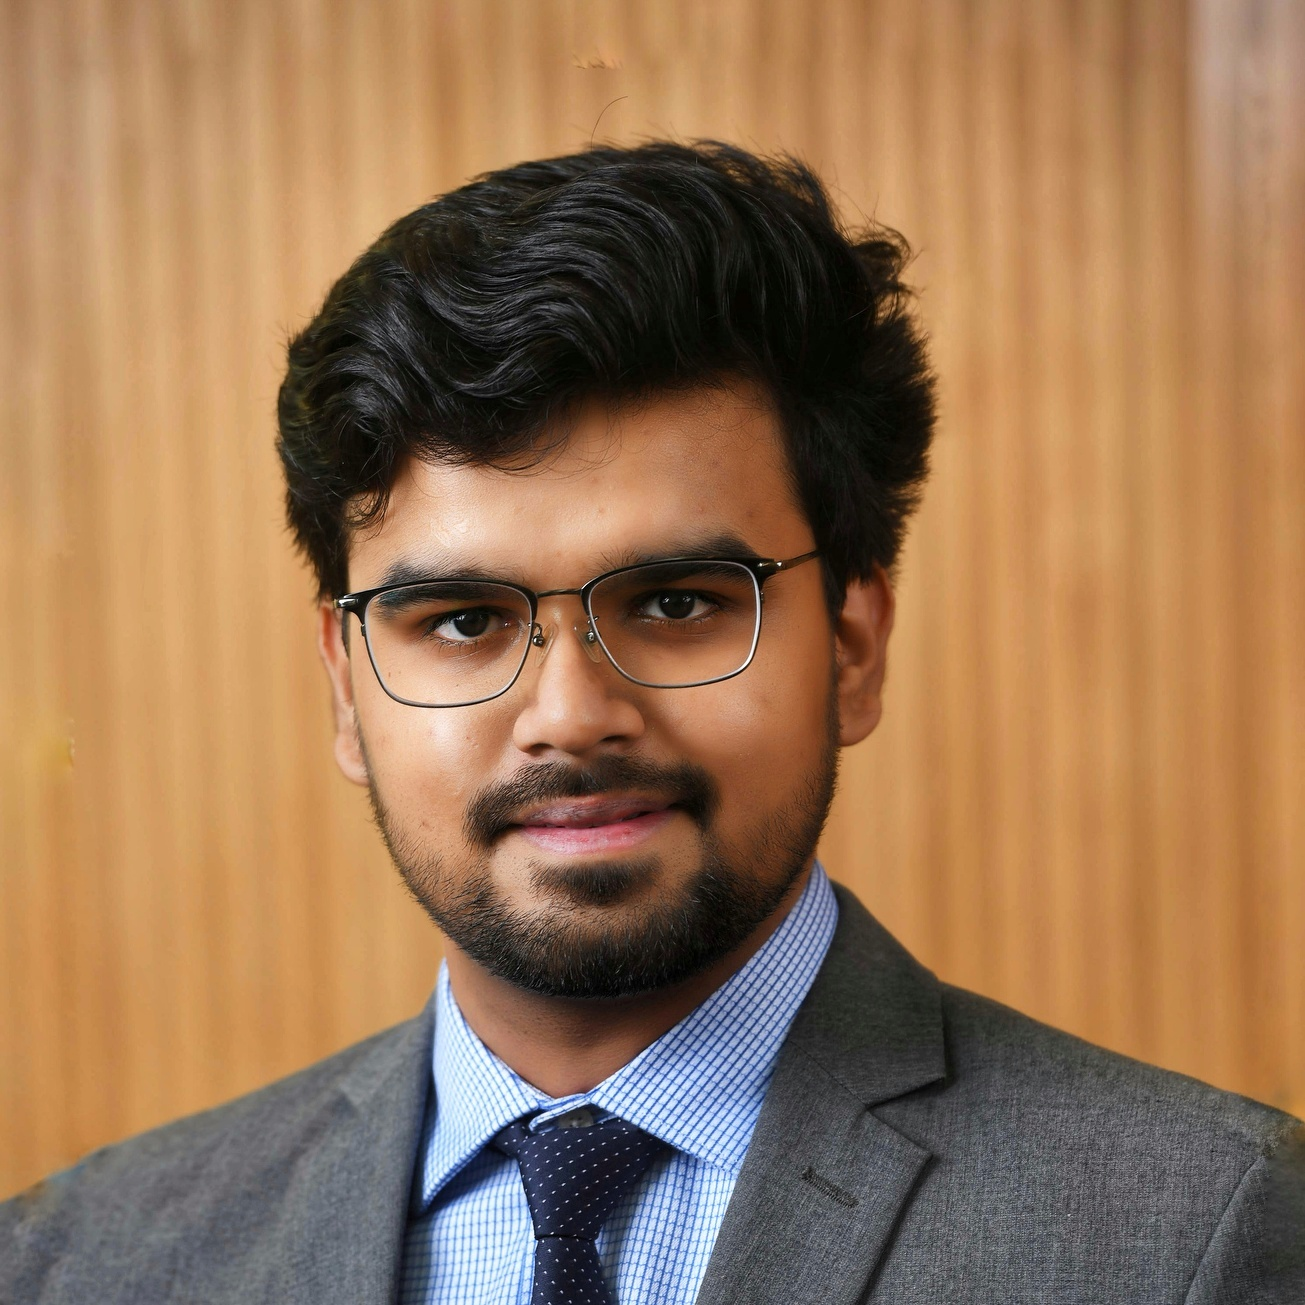
\includegraphics[width=0.5\textwidth,height=\textheight]{Images/Amey.jpeg}

\begin{quote}
Hey There, MBAn folk !! I'm Amey\\
I was born and brought up in India, where I also completed my Bachelor of Engineering in Computer Science, after which I worked as a technology consultant for three years. During my time at Deloitte, I realized my interests lie at the interface of technology and business; And I needed to expand my skills and knowledge in these domains, which is when I decided to join Ross Business School. ~
I wish to leverage data and apply ML/analytical frameworks to derive actionable insights and create value. I enjoy operating far outside my comfort zone and believe in the power of incremental improvements.\\
Feel free to reach out; I am always happy to help :)
\end{quote}

\begin{quote}
``Data is just summaries of thousands of stories - tell a few of them to the world, and you are a data analyst.''
\end{quote}

\hypertarget{eunguy-lee-1}{%
\section*{Eunguy Lee}\label{eunguy-lee-1}}
\addcontentsline{toc}{section}{Eunguy Lee}

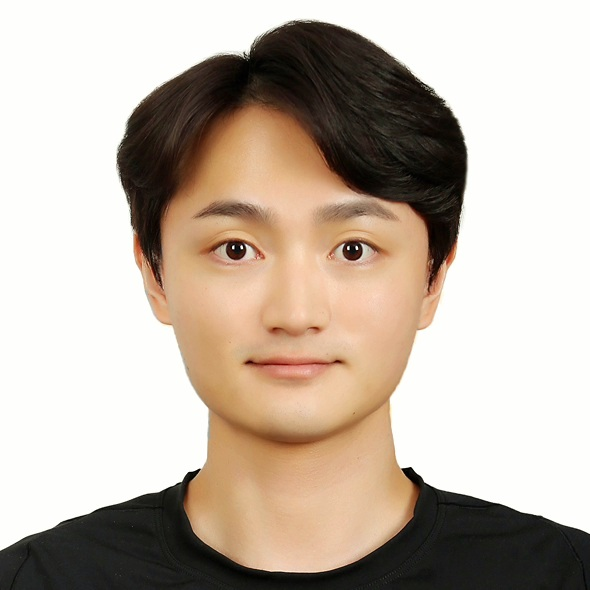
\includegraphics[width=0.5\textwidth,height=\textheight]{Images/Eunguy.jpg}

\begin{quote}
Hello everyone! This is Eunguy.\\
I was born in 1996 and grew up in South Korea. I went to Michigan State University and studied Supply Chain Management. After my junior year in college, I went back to South Korea to serve military as an operations sergeant for about two years. After the military experience, I finished my bechelor degree with online courses from MSU because of the pandemic. Meanwhile, I felt the need of capability handling data so I applied for graduate school with Business Analytics major.
\end{quote}

\begin{quote}
At this point at Ross, I am so exciting to build my network and equip myself with useful tools, such as Python, R, and SQL. As a business person, I am not used to these computer skills. However, someone said ``the pain that doesn't kill you will make you stronger.'' I believe putting my time and effort for the next 10 months will develop my ability as a business analyst. I hope this career handbook brings some insights for you.
\end{quote}

\hypertarget{snow-shen-1}{%
\section*{Snow Shen}\label{snow-shen-1}}
\addcontentsline{toc}{section}{Snow Shen}

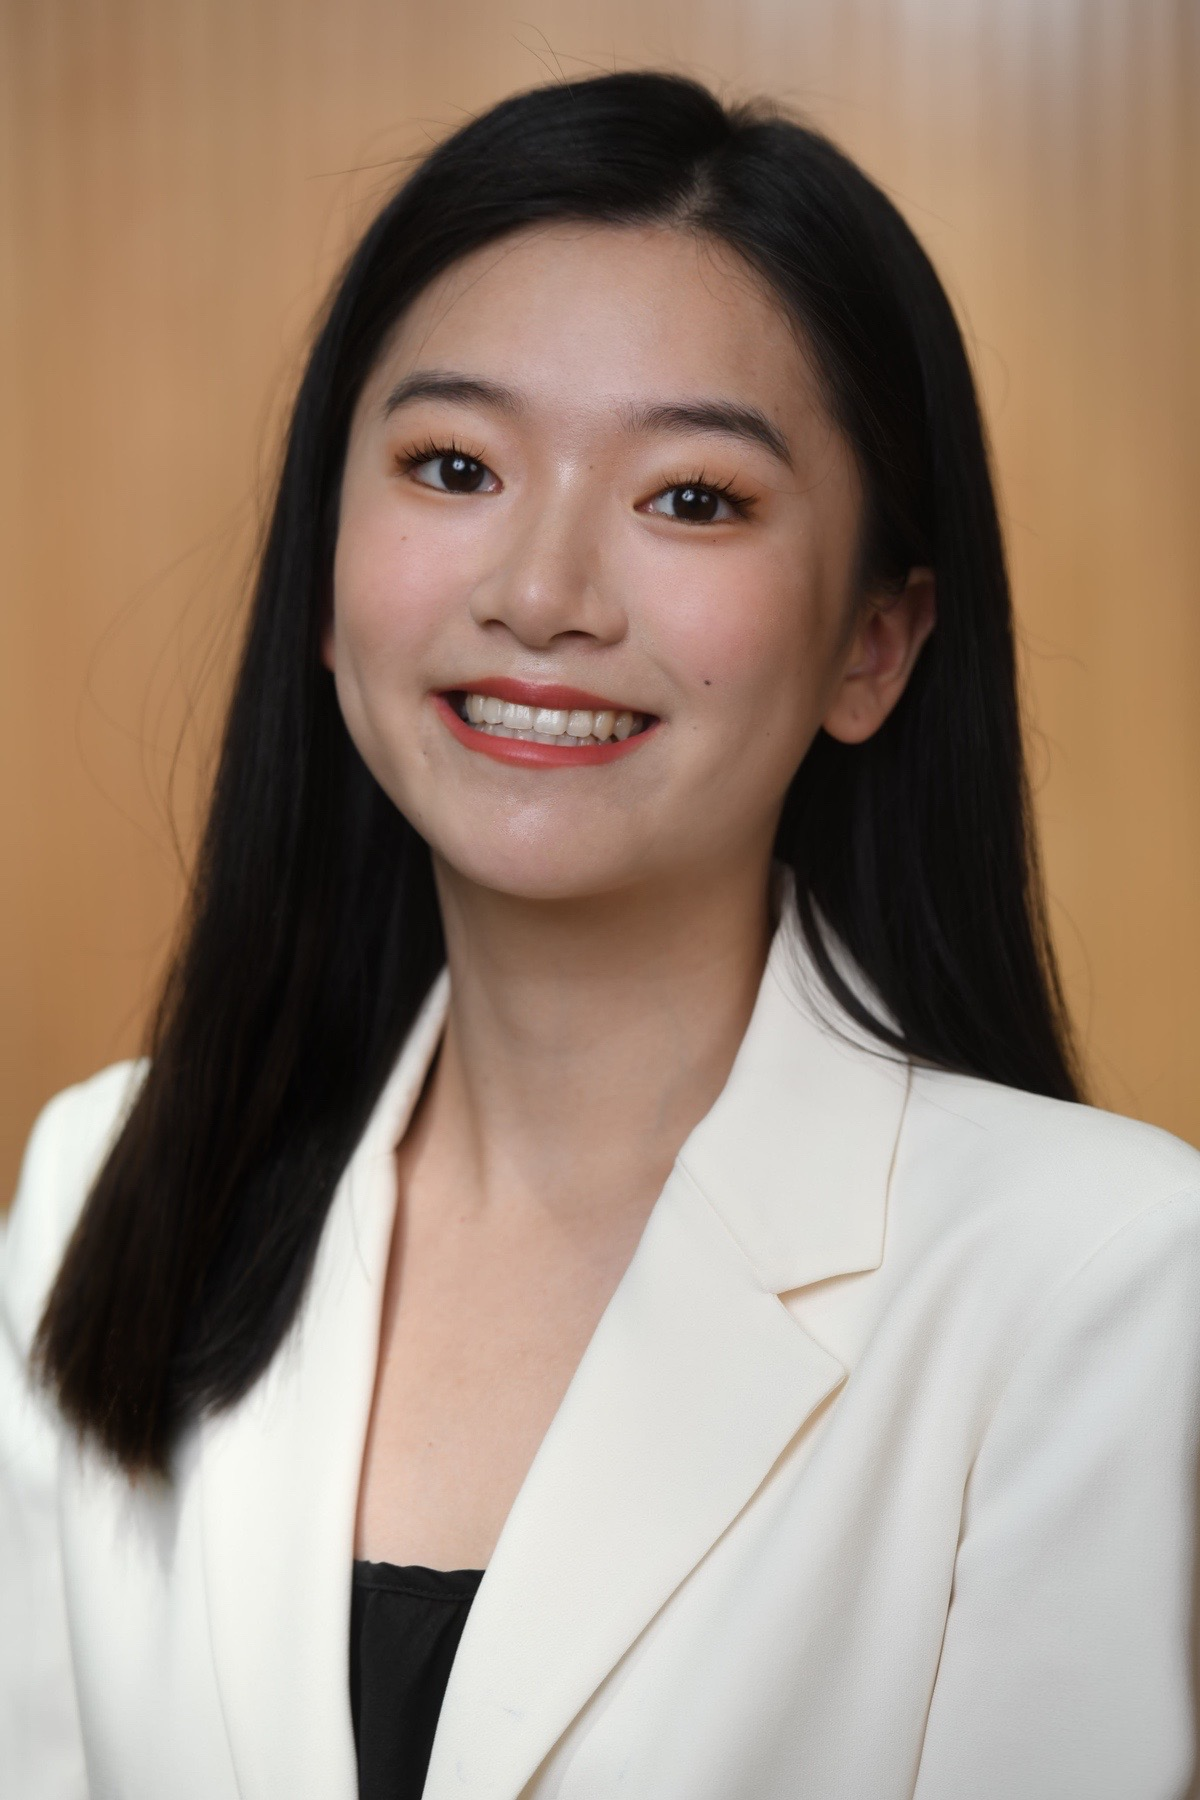
\includegraphics[width=0.5\textwidth,height=\textheight]{Images/Snow.png}

\begin{quote}
Hi, I'm Snow! I come from a southern city in China called Hangzhou. It's warm there and seldomly snows. Every winter, I waited for snow and hoped the world can be covered in white when I wake up. That's why my parents gave me the English name Snow. I went to US in 2019 for my undergrad study. Boston was my destination due to the attractiveness of snow. I spent three years at Boston and then moved to Ann Arbor for graduate study. People hate the long winter here, but I am looking forward to it!
\end{quote}

\hypertarget{mary-silvio-1}{%
\section*{Mary Silvio}\label{mary-silvio-1}}
\addcontentsline{toc}{section}{Mary Silvio}

\includegraphics[width=0.5\textwidth,height=\textheight]{Images/Mary.JPEG}

\begin{quote}
I am a self-proclaimed true Midwestern girl that grew up in Livonia, Michigan (perfectly halfway between Ann Arbor and Detroit). I graduated from the University of Michigan College of Engineering in Spring 2022 with a B.S.E. in Chemical Engineering and am a current Master's of Business Analytics student at the Stephen M. Ross School of Business. If there is one thing I took away from my undergraduate years, it is that the world will never run out of ways to improve, and thus never run out of problems to solve. Pushing the bounds of knowledge is what allows us to improve the systems around us, and that is why I value the potential of harnessing data - bringing me to the MBAn program to build my analytic skills to give data power.
\end{quote}

\begin{quote}
I have experience working in Chemical Manufacturing, Engineering Research, and Higher Education. Outside of school, I love going to SoulCycle, going on walks with friends, watching Detroit sports, trying new coffee shops, and cooking! It is my dream to be an analyst by day, and cycling instructor by night.
\end{quote}

\hypertarget{ziye-wang-1}{%
\section*{Ziye Wang}\label{ziye-wang-1}}
\addcontentsline{toc}{section}{Ziye Wang}


\includegraphics[width=0.5\textwidth,height=\textheight]{Images/Siye.jpg}

\begin{quote}
My name is Ziye Wang, from Beijing, China. I graduated from the Central University of Finance and Economics in China, majoring in Financial Engineering.After graduation, I joined Capgemini Invent as an associate consultant, focused on auto and digital transformation.
\end{quote}

\begin{quote}
Something interesting about me I'd like to share with you:
I like drinking more than I like soup
I have 3 cute little nephews and my favorite thing to do on weekends is to play with my little nephew
I'm a Cancer girl but I'm more of a Leo
I lost weight for 5 years but never succeeded
\end{quote}

\begin{quote}
I'm very happy to be part of the Ross community. Hopefully our work will be helpful to everyone.
\end{quote}

\hypertarget{references}{%
\chapter*{References}\label{references}}
\addcontentsline{toc}{chapter}{References}

\begin{itemize}
\tightlist
\item
  \url{https://365datascience.com/career-advice/career-guides/data-scientist-2021/}
\end{itemize}

\hypertarget{hello-bookdown}{%
\section*{Hello bookdown}\label{hello-bookdown}}
\addcontentsline{toc}{section}{Hello bookdown}

All chapters start with a first-level heading followed by your chapter title, like the line above. There should be only one first-level heading (\texttt{\#}) per .Rmd file.

\hypertarget{a-section}{%
\section{A section}\label{a-section}}

All chapter sections start with a second-level (\texttt{\#\#}) or higher heading followed by your section title, like the sections above and below here. You can have as many as you want within a chapter.

\hypertarget{an-unnumbered-section}{%
\subsection*{An unnumbered section}\label{an-unnumbered-section}}
\addcontentsline{toc}{subsection}{An unnumbered section}

Chapters and sections are numbered by default. To un-number a heading, add a \texttt{\{.unnumbered\}} or the shorter \texttt{\{-\}} at the end of the heading, like in this section.

\hypertarget{challenges-for-international-students}{%
\chapter*{Challenges for International students}\label{challenges-for-international-students}}
\addcontentsline{toc}{chapter}{Challenges for International students}

\hypertarget{sponsorship}{%
\section{Sponsorship}\label{sponsorship}}

\hypertarget{h1b-process}{%
\section{H1B process}\label{h1b-process}}

\hypertarget{resources}{%
\section{Resources}\label{resources}}

\hypertarget{recruiting-process}{%
\chapter*{Recruiting Process}\label{recruiting-process}}
\addcontentsline{toc}{chapter}{Recruiting Process}

\hypertarget{resume-preparation-process}{%
\section{Resume preparation process}\label{resume-preparation-process}}

\hypertarget{whats-in-your-toolbox}{%
\subsection{What's in your ``Toolbox''}\label{whats-in-your-toolbox}}

\hypertarget{what-resources-does-oym-provide}{%
\subsection{What resources does OYM provide?}\label{what-resources-does-oym-provide}}

\hypertarget{list-and-links-to-useful-resources-to-look-out-for}{%
\subsection{List and links to useful resources to look out for}\label{list-and-links-to-useful-resources-to-look-out-for}}

\hypertarget{interview-preparation-process}{%
\section{Interview preparation process}\label{interview-preparation-process}}

\hypertarget{sample-questions}{%
\subsection{Sample questions}\label{sample-questions}}

\hypertarget{mock-interviews}{%
\subsection{Mock interviews}\label{mock-interviews}}

\hypertarget{interview-prep-books-reaching-out-to-full-time-mbaconsulting-club-and-mm-who-has-experience}{%
\subsection{Interview Prep books (reaching out to full-time mba(consulting club) and mm (who has experience))}\label{interview-prep-books-reaching-out-to-full-time-mbaconsulting-club-and-mm-who-has-experience}}

\hypertarget{expected-timeline-and-plan}{%
\section{Expected timeline and plan}\label{expected-timeline-and-plan}}

\hypertarget{schedule-for-different-industries-recruiting-practices}{%
\subsection{Schedule for different industries recruiting practices}\label{schedule-for-different-industries-recruiting-practices}}

\hypertarget{deadlines-to-give-yourself-to-be-prepared-and-proactive}{%
\subsection{Deadlines to give yourself to be prepared and proactive}\label{deadlines-to-give-yourself-to-be-prepared-and-proactive}}

\hypertarget{time-management-for-balancing-recruiting-and-classes-simultaneously}{%
\subsection{Time management for balancing recruiting and classes simultaneously}\label{time-management-for-balancing-recruiting-and-classes-simultaneously}}

  \bibliography{book.bib,packages.bib}

\end{document}
